\documentclass{article}
\usepackage[margin=0.7in]{geometry} % change this parameter to enlarge/restrict the margins
\usepackage{amsmath,amsthm,amssymb,amsfonts, fancyhdr, color, comment, graphicx, environ}
\usepackage{xcolor}
\usepackage{mdframed}
\usepackage[shortlabels]{enumitem}
\usepackage{hyperref}
\usepackage{calrsfs}
\usepackage{subfig}
\DeclareMathAlphabet{\pazocal}{OMS}{zplm}{m}{n}
\usepackage{graphicx}
\usepackage{makecell} %table cells
\usepackage{booktabs} %table appearance
\usepackage{caption} %table caption

\renewcommand{\footrulewidth}{0.8pt}
\hypersetup{
	colorlinks=true,
	linkcolor=blue,
	filecolor=magenta,      
	urlcolor=blue,
}

%/ Margin
%/ ##########################
%/\addtolength{\oddsidemargin}{-.7in}
%/\addtolength{\evensidemargin}{-.7in}
%/\addtolength{\textwidth}{1.4in} %/Double of the 2 above
% ###########################

% fancy style 
\pagestyle{fancy}
% remove fancy style from bottom 
\renewcommand{\footrulewidth}{0pt}

\lhead{Group 20}
\rhead{Algorithmic Machine Learning} 

\newcommand{\loss}{L(\theta, a)}
\newcommand{\lossRule}{L(\theta, \delta(x))}
\newcommand{\risk}{R(\theta, \delta)}

%------------------------------------------------
% Bibliography
\usepackage[sorting=none, backend=bibtex]{biblatex}
\addbibresource{ref.bib}
%------------------------------------------------


\begin{document}
	\title{\Large Algorithmic Machine Learning  \\[0.5cm]
	\bf\Large Challenge 1 - Report \\[0.5cm]
	
	\bf\Large Group 20}

\author{\large 
	\begin{tabular}{rl}
		\textbf{Professor:} & Pietro Michiardi \\
		\textbf{Authors:} & Daniele Falcetta \\ & Simone Papicchio \\ & Massimiliano Pronesti \\ & Federico Tiblias
	\end{tabular}
	}
\date{\large \today}

\makeatletter
\begin{titlepage}
	\begin{center}
		{ 
\includegraphics[width=10cm]{assets/eurecom.png}}
		{\ \\ \ \\}
		\vbox{}\vspace{5cm}
		{\@title }\\[3cm]
		{\@author}\\[3cm]
		{\@date\\}
		
	\end{center}
\end{titlepage}
\makeatother
	
\section{Introduction}
With the increasing amount of content and debate on social media platforms such as Twitter, there is an interest in automatically extracting meaning and sentiment from users' posts, to be able to evaluate the aggregate opinion of a large number of users.

The dataset used for this challenge consist of tweets from Figure Eight's Data for Everyone platform. The main task is to classify tweets with positive, neutral, or negative labels. We compare different solutions: from techniques based on word embeddings, to LSTM models, to state-of-the-art approaches using pre-trained transformers.
This challenge proposes the additional task of finding the most important words in a sentence. We propose two approaches: one based on word counts and the other on \textit{Transformers Interpret} and on \textit{Captum} \cite{kokhlikyan2020captum}, a tool and library, respectively, for model interpretability and visualization. 

% In this challenge we also address a further bonus task which consists of detecting the relevant words inside the tweet which are most responsible for the attributed sentiment.


\section{Data Analysis \& Pre-processing}
    \subsection{Data exploration}
    Tweets are, in general, quite far from plain English text, as they usually contain slang, abbreviations, emojis, emoticons and misspellings. Those available in the given dataset are no exception. 
    
    We start our data exploration by studying the label distribution. As we can see from the pie chart in Figure \ref{fig:exploration}, the dataset is slightly imbalanced towards the \textit{neutral} class whereas almost balanced between \textit{positive} and \textit{negative} tweets. A further analysis on the text length distribution of each class reveals that almost each category of tweets has the same one, as shown in Figure \ref{fig:exploration} for the \textit{positive} class.
    In addition, looking at the Wordclouds for the \textit{positive} and \textit{negative} tweets shown in Figure \ref{fig:wordcloud}, we can also notice, as expected, that the most present terms are words like \textit{love}, \textit{good} and \textit{thanks} for the former and \textit{sad}, \textit{work} and \textit{miss} for the latter.   
    
    \begin{figure}[h]%
    \centering
    \subfloat{{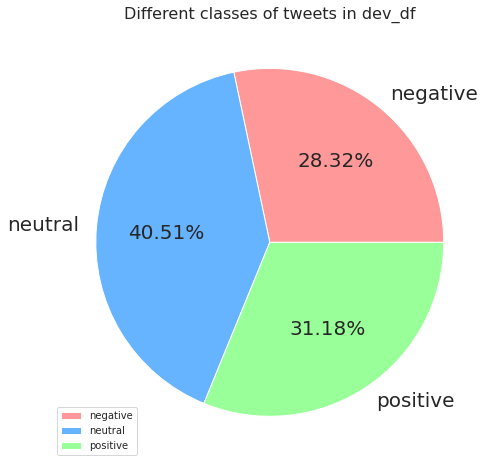
\includegraphics[width=0.3\linewidth]{assets/pietweet.png} }}%
    \qquad
    \subfloat{{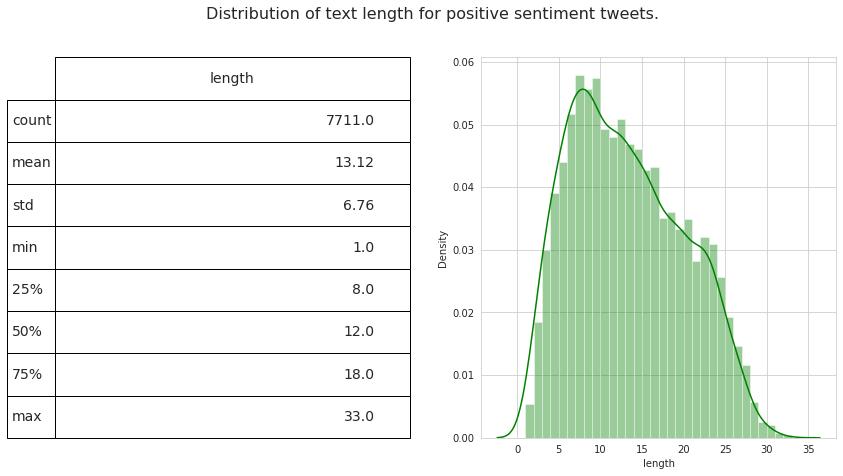
\includegraphics[width=0.5\linewidth]{assets/distriblength.png} }}%
    \caption{Classes and text length distribution in the training dataset }%
    \label{fig:exploration}%
    \end{figure}
    
    \begin{figure}[h]%
    \centering
    \subfloat{{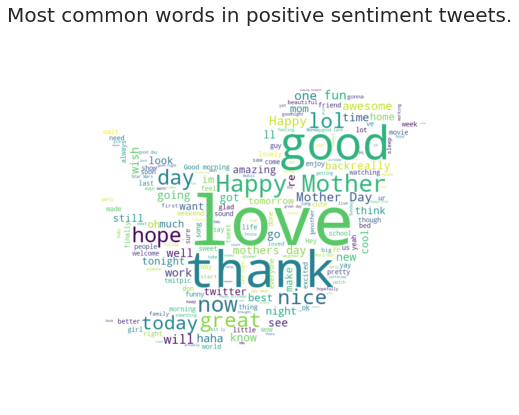
\includegraphics[width=8cm]{assets/wordcloudpos.png} }}%
    \qquad
    \subfloat{{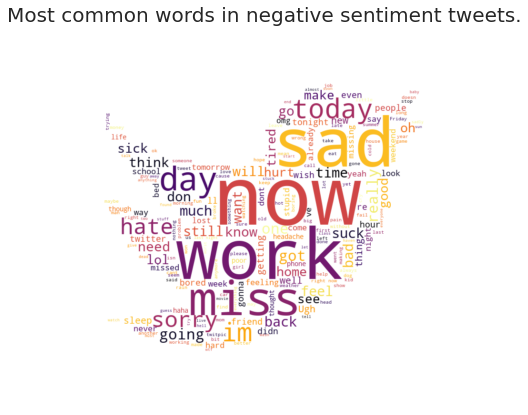
\includegraphics[width=8cm]{assets/wordcloudneg.png} }}%
    \caption{Wordclouds for the training dataset}%
    \label{fig:wordcloud}%
    \end{figure}
    % \begin{center}
    %     \begin{tabular}{cc}
    %     \toprule
    %     \makecell{Feature}& \makecell[t]{Importances} \\
    %     \midrule
    %     \textbf{wrf\_t2\_interpolated}     & \textbf{0.871038}\\
    %     gfs\_temperature\_97500   & 0.034633\\
    %     cmc\_0\_0\_6\_2             & 0.011729\\
    %     climate\_temperature     & 0.010516\\
    %     wrf\_snow                & 0.004567\\
    %     sun\_elevation           & 0.004368 \\
    %     cmc\_0\_0\_7\_2             & 0.004134\\
    %     cmc\_0\_1\_0\_0             & 0.003386\\
    %     gfs\_soil\_temperature    & 0.002967\\
    %     fact\_longitude          & 0.002202\\
    %     \bottomrule
    %     \end{tabular}
    %     \captionsetup{width=0.8\linewidth}
    %     \captionof{table}{The 10 most important features extracted with a Random Forest with 10 trees and max depth equal to 30}
    %     \label{table:featImpo}
    % \end{center}
    
    
    
    \subsection{Pre-Processing}
    \label{pre_processing}
	\begin{itemize}
		\item \textbf{Emojis and Emoticons:} Punctuation marks, letters, and numbers used to create pictorial icons that generally display an emotion or sentiment. We convert them to the equivalent textual representation of the emotion they attempt to convey employing the \textit{emot} library. A complete and more effective parsing required, however, integrating the original dictionary with some missing entries\footnote{the "complete" list is taken from Wikipedia: https://en.wikipedia.org/wiki/List\_of\_emoticons}.
		\item \textbf{Abbreviations and Slang:} Similarly to emojis and emoticons, we do a raw text preprocessing in order to map the most famous slangs and abbreviations with the correct word in regular English.
		\item \textbf{SpellChecker:} Employing the \textit{SpellChecker} library, we attempt to convert misspelled word to correct English.
		\item \textbf{Tokenization:} Tokenization consists in breaking the raw text into small chunks called tokens. Many algorithms use tokens as input to conduct further analysis.
        \item \textbf{Stopwords removal:} Stopwords are a set of commonly used words in any human language. For instance, examples of stopwords in English are: “the”, “is” and “and”. It's therefore a common practice to remove them to allow models to focus on the important words. The stopwords dictionary is taken from the \textit{nltk} library. 
		
		\item \textbf{Stemming \& Lemmatization:} The goal of both method is to reduce inflectional forms and sometimes related forms of a word to a common base form. Stemming uses the stem of the word, while lemmatization uses the context in which the word is being used. 
		
	\end{itemize}
    \subsection{Augmentation}
    While our training dataset contains roughly 25k entries, it still pales in comparison to the huge amount of data transformer models were trained on. To better fine-tune our pretrained models, we try different techniques to increase the number of available datapoints. 
	\begin{itemize}
		\item \textbf{Concatenation:} Build new tweets by concatenating existing ones. Couples are formed randomly and kept only if the tweets have the same label and  the resulting tweet is $< 140$ characters long. This procedure can be repeated producing datasets of increasing size.
		\item \textbf{Backtranslation:} Transformer models are capable of translating back and forth from a language. Due to linguistic differences and imperfections in the model, the backtranslation is not always a perfect replica of the original sentence but maintains the original meaning. We exploit this phenomenon to build new sentences that have the same meaning of the original one, but a different structure. German is chosen for this task as it's the closest language to English that also has readily available pre-trained models. In particular, we rely on Hugging Face's \texttt{Helsinki-NLP/opus-mt-en-de} and \texttt{Helsinki-NLP/opus-mt-de-en}. Generated sentences are kept only if they are different than the original ones.
	\end{itemize}

    \subsection{Word Embeddings}
    Word embeddings are a type of representation that allows words with similar meaning to have a similar representation\footnote{Distributional Hypothesis: given a word, we look for the semantically related words that are nearby}. Before embedding our data we perform all preprocessing steps described in Section \ref{pre_processing}.
    
    \begin{itemize}
        \item \textbf{Word2Vec:} Two-layer neural network that processes text by “vectorizing” words.  Word2vec groups the vectors of similar words together in a vector space by detecting similarities. For this task, we train\footnote{\textit{context window 5, negative sampling 10, skip-gram model 1, vector size 663}} the neural network\footnote{\textit{https://radimrehurek.com/gensim/models/word2vec.html}} on the processed tweet, creating a feature space of size 18964 unique tokens x 663 vector size. The main drawbacks of this representation are that it is unable to model the sequences of word (solved by LSTM), it ignores the global word co-occurrence (solved by GloVe), not designed for encoding contextual representation (solved by Transformers)
        \item \textbf{GloVe\cite{glove}:} Unsupervised learning algorithm for obtaining vector representations for words. Training is performed on aggregated global word-word co-occurrence statistics from a corpus, and the resulting representations showcase linear substructures of the word vector space. We download the embedding containing the glove vectors trained on the Wikipedia and GigaWord dataset. The feature space size is 400000 unique tokens x 50 vector size. The main drawback of this embedding is that it is not trained on our tweets, i.e. most of the words are completely unknown to the space.
    \end{itemize}

\section{Models}
    Transformers are undoubtedly the gold standard for many NLP tasks including sentiment analysis. Nevertheless, we also try different approaches to see how they compare  with the state of the art.
    
    Scores are computed by first splitting the labelled data in development and validation datasets (80/20 random split), then training on the development part, and finally assessing performances on the unseen validation subset. If the model reaches satisfying results is then applied on the unlabelled test dataset and predictions are uploaded on Kaggle.
	\begin{itemize}
		\item \textbf{KNN/Random Forest/CatBoost:} We exploit the embedded text to attempt tackling the sentiment analysis problem in a "classical" machine learning fashion, using it as training data to be fed to a KNN, a Random Forest and a Catboost classifier.
		\item \textbf{Convolutional LSTM:} This architecure is used with both Word2vec Tab.\ref{table:lstm_word2vec} and GloVe Tab.\ref{table:lstm_gloVe}. In both cases, the architecture takes as input the pre-processed sentence already tokenized. Each token is mapped into the respective feature vector. The output of the embedding is passed to a Spatial Dropout with different percentages for the architectures. A convolutional layer with 64 kernels size 5 creates the input for the LSTM. Before the classification, there are several fully connected layer. The tables below show the differences between the architectures.
		\item \textbf{Transformer:} A transformer is a deep learning model which adopts the mechanism of self-attention, differentially weighting the significance of each part of the input data. Unlike RNNs, transformers process the entire input all at once. They do so through the attention mechanism, a technique able to enhance some parts of the input data while diminishing others, mimicking how real brains focus attention on specific aspects of information. In particular we use  "Twitter-roBERTa-base for Sentiment Analysis", a 125M parameter transformer model pretrained on the TweetEval dataset\cite{Chefer_2021_CVPR}, which we further fine-tune for our task.
	\end{itemize}

% \vspace{0.5cm}    
% \setlength{\tabcolsep}{8pt}
% \hspace{-0.5cm}
\begin{minipage}[c]{0.5\textwidth}
\centering
    \begin{tabular}{lccl}
        \toprule
        \makecell{Layer}              & \makecell[l]{Output shape} & \makecell[t]{Param \#}\\
        \midrule
        InputLayer                      &  [bs, 33]      & 0      \\
        Embedding                       &  [bs, 33, \textbf{663}]  &  \textbf{131,532,570}           \\
        Spatial Dropout \textbf{(0.6)}                &  [bs, 33, 663]  &  0            \\
        Conv1D                          & [bs, 29, 64]    &  212,224             \\
        Dropout (0.6)                        & [bs, 29, 64]    & 0               \\
        Bidirectional LSTM              & [bs, \textbf{128}]       & \textbf{98.816}               \\
        Dropout  \textbf{(0.4)}                        & [bs, 128]      & 0         \\
        Dense                           & [bs, \textbf{512}]      & \textbf{131,584}\\
        Dropout  \textbf{(0.4)}                        & [bs, 512]      & 0            \\
        Dense                           & [bs, 512]       & 524,800        \\
        Dense                           & [bs, 3]       & 1,539       \\
        \bottomrule
    \end{tabular}
    \captionsetup{width=0.8\linewidth}
    \captionof{table}{LSTM Architecture with Word2Vect embedding, 132,501,533 trainable parameters}
    \label{table:lstm_word2vec}
\end{minipage}
\begin{minipage}[c]{0.5\textwidth}
\centering
    \begin{tabular}{lccl}
        \toprule
        \makecell{Layer}              & \makecell[l]{ Output shape} & \makecell[l]{Param \#}\\
        \midrule
        InputLayer                      &  [bs, 33]      & 0      \\
        Embedding                       &  [bs, 33, \textbf{50}]  &  \textbf{9,919,500}           \\
        Spatial Dropout \textbf{(0.8)}                &  [bs, 33, 50]  &  0            \\
        Conv1D                          & [bs, 29, 64]    &  \textbf{16,064}              \\
        Dropout (0.6)                        & [bs, 29, 64]    & 0               \\
        Bidirectional LSTM              & [bs, \textbf{256}]       & \textbf{197,632}               \\
        Dropout  \textbf{(0.6)}                        & [bs, 256]      & 0         \\
        Dense                           & [bs, \textbf{1024}]      & \textbf{263,168}\\
        Dropout  \textbf{(0.6)}                        & [bs, 1024]      & 0            \\
        Dense                           & [bs, 512]       & 524,800        \\
        Dense                           & [bs, 3]       & 1,539       \\
        \bottomrule
    \end{tabular}
    \captionsetup{width=0.8\linewidth}
    \captionof{table}{LSTM architecture with the GloVe embedding, 10,922,703 trainable parameters.}
    \label{table:lstm_gloVe}
\end{minipage}


\section{Results}
\begin{itemize}
		\item \textbf{KNN/Random Forest/CatBoost:} As expected, these approaches proved unsuccessful, with a validation score below 60\%.
		\item \textbf{Conv LSTM:} The results are heavily influenced by the selected feature space. The Word2vec LSTM is able to obtain almost 88\% of training accuracy but only 68\% for validation accuracy. We try addressing the overfitting problem by introducing several dropout layers. However, this solution combined with GloVe produces even worse results, achieving a score in the ballpark of 40\% both in training and validation sets. This low accuracy is mostly caused by the domain adaptation  problem, as we download a feature space pretrained on Wikipedia + GigaWord dataset, which is not similar to our dataset. 
		\item \textbf{Transformer:} As expected, transformer models outperform all other approaches. This can be attributed to their internal complexity and extensive training\cite{Chefer_2021_CVPR}. We also point out that preprocessing to remove emoticons, abbreviations, slang, misspellings and URLs make the model perform slightly better than without.
\end{itemize}
	
Interestingly enough, data augmentation does not provide any meaningful improvements to any model.

\section{Bonus Task}
With the increase in model complexity and the resulting lack of transparency, model interpretability methods have become increasingly important. We address two methodologies to extract the important words in a piece of text:
\begin{itemize}
		\item \textbf{Count-based scoring:} For each word, count its occurrences in  positive tweets and subtract its occurrences in negative tweets. Keep only words with a high or low enough score as they correlate more with one class of tweets. Note that this method is only able to explain positive or negative words, but not neutral ones. It results in a 0.13 mean Jaccard similarity score.
		
		\item \textbf{Transformers Interpret and Captum:} libraries providing state-of-the-art algorithms, including Integrated Gradients, to perform model explainability. For each tweet, the model is able to recognize, through the use of a threshold, the words that best explain the sentiment for each class. The higher the score, the more important is that term. 
        By analyzing the results for our tweets we can notice that the model is able to select the right terms when the sentence is short and the sentiment is clearly defined while it struggles when the tweet is not written in plain English but it contains some expression typical of a message. In Figure \ref{fig:Explainability Score} is shown a negative example. Even if this approach uses the power of the self attention layers, it is not able to outperform the Count-based scoring. This happens because some words are divided in chunks to increase the accuracy of the model which leads, for instance, to the split of the word \textit{"belgium"} in \textit{"bel-g-ium"} so that we end up with high manually checked results but poor Jaccard score (only 32\%) 
\end{itemize}

  \begin{figure}[h]
        \hspace{.45cm}
        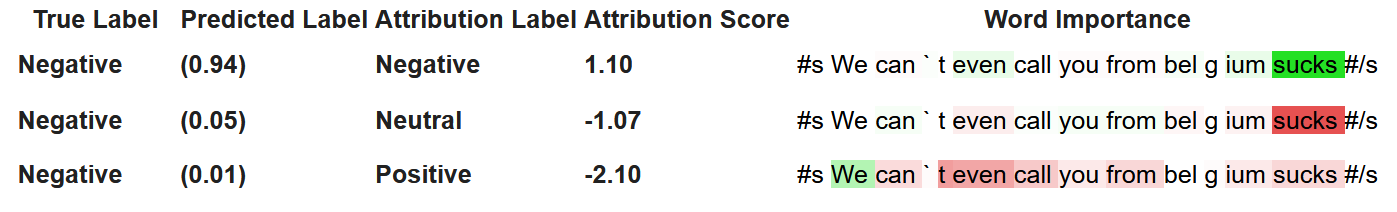
\includegraphics[width=\linewidth]{assets/visualizations.png}
        \caption{An example of transformers explainability. The greener the background, the more important the word is for the predicted label. The other way around with red. Namely, the word "sucks" heavily moves the prediction towards the negative class and away from the neutral class. Label attribution score represents the confidence of the model interpreted as: high positive or negative values as confident and values close to zero as not confident.   }
        \label{fig:Explainability Score}
    \end{figure}

\section{Conclusions}
We showed an interesting comparison of various methods for sentiment analysis, confirming transformer models as the state-of-the-art. Our results show that, while the classical ML approaches are too simple for a complex task like the \textit{Tweets Sentiment Analysis}, different types of embedding with ConvLSTM perform very well during the training phase but are not able to generalize over unseen tweets.
On the other hand, transformers outperform all the other approaches but they need to be fine-tuned and require a good preprocessing to achieve an higher accuracy. This is due to the fact that our dataset is not written in plain English but contains lots of slang words and abbreviation typical of the internet world.
To overcome the overfitting problem, present in all the tested models, a possible solution could be to increase the training dataset or add some regularizing techniques such as a dropout.
%Other improvements are possible by testing different and larger transformers that fit better our complex dataset




%% display bibliography at the end
\printbibliography
\end{document}